%Note di Ingegneria del Software
%Sommario: Idea modello SPY, CMMI

\cornell{Modello SPY}{ 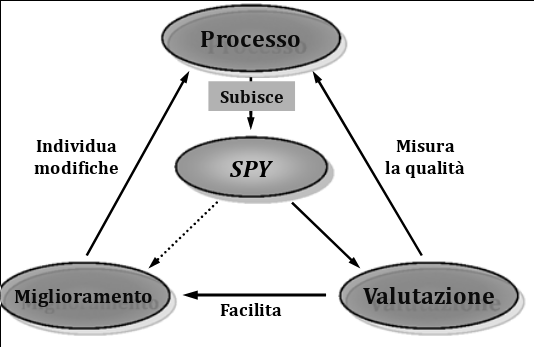
\includegraphics[scale=0.5]{images/59.png} }

\cornell{CMMI}{ \begin{description}
\item [Capability] Misura l'adeguatezza di un processo per gli scopi assegnati.\\
Caratteristica di un processo, preso da solo.\\
Determina l'intorno del risultato raggiungibile dal processo
\item [Maturity] Misura quanto (e quanto bene) l'azienda è governata dal suo sistema di processi.\\
È una caratteristica di un insieme di processi.\\
Risulta dall'effetto combinato delle capability dei processi considerati.
\item [Model] Criteri per valutare il grado di qualità dei processi dell'azienda
\item [Integration] Architettura di integrazione delle diverse discipline
\end{description} }

\cornell{Processi e Capability}{Un processo a basso livello di capability: \begin{itemize}
\item Dipende da chi lo attua
\item È definito ed attuato in modo opportunistico
\item Ha esito, avanzamento e qualità difficili da prevedere
\item Porta a compromessi tra qualità e funzionalità
\end{itemize}\\
Mentre dei processi ad alto livello di capability sono eseguiti da tutti quanti in modo disciplinato, sistematico e quantificabile.}

\cornell{Governance}{Intelligenza dei processi di una organizzazione (in termini di Efficacia, Efficienza, Manutenzione e Visione)\\
È un'attività continua}

\cornell{Livelli di Maturità CMMI}{ \begin{enumerate}
\item Initial - I processi sono imprevedibili, mal controllati e reattivi.\\
Inoltre i processi sono non sistematici e non quantificabili.
\item Managed - I processi sono definiti per progetto, e sono solitamente reattivi (Qui applico "Do" del PDCA)
\item Defined - Processi sono caratterizzati per organizzazione e sono proattivi invece di reattivi (Si applica "Plan" del PDCA)
\item Quantitatively Managed - I processi sono quantificabili e controllati (Qui si applicano "Plan" e "Check" del PDCA)
\item Optimizing - Ci si concentra sul miglioramento, applicando completamente il PDCA
\end{enumerate}}

\cornell{Produttività}{Quantità di risorse usate per produrre una unità di prodotto \textbf{Conforme} (meno è meglio)}

\cornell{Costi e benefici del CMMI}{ \begin{itemize}
\item Si ha un aumento della produttività
\item Miglioramento dell'identificazione dei difetti nelle prime fasi di produzione
\item Riduzione del time-to-market
\item Riduzione dei difetti rilevati sul campo
\item Ritorno dell'investimento di circa 5 volte
\end{itemize}}

\cornell{ISO/IEC 15504}{"Abolisce" la maturity basata sul "voto peggiore" (Il bottom) di CMMI e consente alle organizzazioni di vedersi con più sfaccettature, invece di focalizzarsi sul peggio.\\
È più complesso del CMMI ma consente di avere una visuale più granulare dello stato delle capability dei processi, uno ad uno.}
